%!TEX program = xelatex
\documentclass[UTF8,zihao=5]{ctexart} %ctex包的article


\usepackage[hidelinks]{hyperref}%超链接,自动加到目录里面



\title{{\bfseries\rmfamily\Huge{高等流体力学\hspace{1em}\\第3次阅读报告}}}
\author{周涵宇 2022310984}
\date{}

\usepackage[a4paper]{geometry}
\geometry{left=0.75in,right=0.75in,top=1in,bottom=1in}%纸张大小和页边距

\usepackage[
UseMSWordMultipleLineSpacing,
MSWordLineSpacingMultiple=1.5
]{zhlineskip}%office风格的行间距

\usepackage{fontspec}
\setmainfont{Times New Roman}
\setsansfont{Source Sans Pro}
\setmonofont{Latin Modern Mono}
\setCJKmainfont{SimSun}[AutoFakeBold=true]
% \setCJKmainfont{仿宋}[AutoFakeBold=true]
\setCJKsansfont{黑体}[AutoFakeBold=true]
\setCJKmonofont{DengXian}[AutoFakeBold=true]

\setCJKfamilyfont{kaiti}{楷体}
\newfontfamily\CM{Cambria Math}


% \usepackage{indentfirst} %不工作 怎样调整ctex的段首缩进大小呢

\usepackage{fancyhdr}
\pagestyle{fancy}
\lhead{
    \CJKfamily{kaiti}{
        高等流体力学作业\hspace{6em}
        班级\ \ 航博221\hspace{6em}
        学号\ \ 2022310984\hspace{6em}
        姓名\ \ 周涵宇
        }
}
\chead{}
\rhead{}
\lfoot{}
\cfoot{\thepage}
\rfoot{}
\renewcommand{\headrulewidth}{0.5pt} %改为0pt即可去掉页眉下面的横线
\renewcommand{\footrulewidth}{0pt} %改为0pt即可去掉页脚上面的横线
\setcounter{page}{1}


% \usepackage{bm}

\usepackage{amsmath,amsfonts}
\usepackage{array}
\usepackage{enumitem}
\usepackage{unicode-math}

% \usepackage{titlesec} % it subverts the ctex titles
\usepackage{titletoc}


% titles in toc:
\titlecontents{section}
              [2cm]
              {\sffamily\zihao{5}\mdseries}%
              {\contentslabel{3em}}%
              {}%
              {\titlerule*[0.5pc]{-}\contentspage\hspace*{1cm}}

\titlecontents{subsection}
              [3cm]
              {\rmfamily\mdseries\zihao{5}}%
              {\contentslabel{3em}}%
              {}%
              {\titlerule*[0.5pc]{-}\contentspage\hspace*{1cm}}

\titlecontents{subsubsection}
              [4cm]
              {\rmfamily\mdseries\zihao{5}}%
              {\contentslabel{3em}}%
              {}%
              {\titlerule*[0.5pc]{-}\contentspage\hspace*{1cm}}
\renewcommand*\contentsname{\hfill \sffamily\mdseries 目录 \hfill}

\ctexset{
    section={   
        % name={前面,后面},
        number={\arabic{section}.},
        format=\sffamily\raggedright\zihao{4}\mdseries,
        indent= {0em},
        aftername = \hspace{0.5em},
        beforeskip=1ex,
        afterskip=1ex
    },
    subsection={   
        % name={另一个前面,另一个后面},
        number={\arabic{section}.\arabic{subsection}.}, %如果只用一个数字而非1.1
        format=\rmfamily\raggedright\mdseries\zihao{5},%正体字体,不加粗,main字体,五号字
        indent = {2em}, %缩进
        aftername = \hspace{0.5em},
        beforeskip=1ex,
        afterskip=1ex
    },
    subsubsection={   
        % name={另一个前面,另一个后面},
        number={\arabic{section}.\arabic{subsection}.\arabic{subsubsection}.}, %默认的 1.1.1
        format=\rmfamily\raggedright\mdseries\zihao{5},%无衬线字体,加粗,sans字体,五号字
        indent = {2em}, %缩进
        aftername = \hspace{0.5em},  %名字和标题间插入字符(此处是空白)
        beforeskip=1ex, %空行
        afterskip=1ex
    }
}

\usepackage{float}
\usepackage{graphicx}
\usepackage{multirow}
\usepackage{multicol}
\usepackage{caption}
\usepackage{subcaption}
\usepackage{cite}


%part、section、subsection、subsubsection、paragraph、subparagraph
\newcommand{\bm}[1]{{\mathbf{#1}}}
\newcommand{\trans}[0]{^\mathrm{T}}
\newcommand{\tran}[1]{#1^\mathrm{T}}
\newcommand{\hermi}[0]{^\mathrm{H}}
\newcommand{\conj}[1]{\overline{#1}}
\newcommand*{\av}[1]{\left\langle{#1}\right\rangle}
\newcommand*{\avld}[1]{\frac{\overline{D}#1}{Dt}}
\newcommand*{\pd}[2]{\frac{\partial #1}{\partial #2}}
\newcommand*{\pdcd}[3]{\frac{\partial^2 #1}{\partial #2 \partial #3}}
\newcommand*{\inc}[0]{{\Delta}}

\newcommand*{\uu}[0]{\bm{u}}
\newcommand*{\vv}[0]{\bm{v}}
\newcommand*{\g}[0]{\bm{g}}
\newcommand*{\nb}[0]{{\nabla}}



\begin{document}

\maketitle
\thispagestyle{fancy}


% \begin{center}
%     \rmfamily
%     \tableofcontents\setcounter{page}{0}
% \end{center}
% \thispagestyle{empty} % 目录
% \newpage %换页

阅读文献:A vortex sheet based analytical model of the curled wake behind yawed wind turbines\cite{bastankhah2022vortex}
(面涡近似模型下的偏航风机尾迹解析模型)。


\section{研究背景和意义}
风能领域中各种流体力学现象的解析模型在流体的基础理解以及风场布局优化设计控制方面发挥着重要作用。
典型的例子之一,是风场布局优化中常用的风力涡流尾迹模型。
例如,在经典的Jensen模型中,假设涡流尾迹呈线性扩展且具有帽状形状。
最近的模型使用了更加真实的涡流尾迹横截面,其中包括高斯分布的模型。

风能领域中的解析性尾迹模型在基础理解、
风场设计和控制方面起着重要作用。
其中,尾迹减缓策略的实施中解析性模型尤其有用,
尾迹转向作为一种重要的控制方法,
可增加风场的发电功率。
简而言之,就是风场前排的风机有意识地以偏航条件运行,
将其尾迹从下风风机中偏转。
尽管这会降低偏航风机的发电功率,但研究表明,
由于下风风机产生更多的功率,
整个风场的效率可以提高。
偏航风机尾迹流动具有复杂的特征,使其模化比非偏航情况更具挑战性。
偏航风机尾迹最著名的流体动力学特征之一是其卷曲的横截面形状(即肾形横截面)。
这种形状是由反向旋转的涡对(CVP)的作用产生的。
反向旋转的涡对通常是在流向垂直方向上施加空间横流变化时产生的,
其中最著名的的例子之一是来自有限展长机翼的尾涡,
其卷起形成涡对,
即机翼尾涡。

捕捉偏航风机尾迹的卷曲形状非常重要,
因为卷曲会影响尾迹与下风风机的有效重叠程度,从而影响预测的发电量。
然而,文献中关于卷曲尾迹形状的模型需要进行数值积分,而现有的解析尾迹模型
无法捕捉到尾迹形状的这种变形。
解析表达模型可以简单和明确的形式中表示流动趋势。
除了计算成本低之外,
解析流动模型通常能够揭示流动物理的其他现象,
这些现象可能在使用数值模拟工具时不明显。
因此,本文开发了一种解析模型,
用于预测偏航风机后方尾迹的位移和形状变形。
本文的模型受到二维涡面的先前研究启发。
本文的解析模型预测了从偏航转子周围脱落的涡面在下游传输时的位移和变形。
然后,涡面模型与下游尾迹速度损失的演化模型相结合,
预测了卷曲尾迹的形状和偏航风机下风处的速度分布。

总体来说,本文将解析的面涡模型应用于偏航风机场景,
得到一个容易计算的尾迹预测模型,用于预测弯曲形状的
偏航风机尾迹。
这对风机建设控制、提高发电效率以及理解风机流动现象具有多方面意义。



\section{面涡演化模型}

\renewcommand{\rm}{}

本研究仅对脱落涡旋的流向分量进行建模,
因为侧向尾迹偏转和尾迹横截面的变形主要是由流向分量诱导的速度引起的。
涡面由半无限的流向涡线组成。
为了能够解析求解控制方程,
假设涡面是平面的,
并且其组成的涡线是无限长的,
而非半无限长,这种近似在距离原点越远时改进效果越好。

定义$(x,y,z)$为原点是风机中心的坐标系统,$x$是流向,
同时$yz$面内定义极坐标$(r,\theta)$,中心$C$在涡面中心。
$(x_c,y_c,z_c)$是$C$的坐标。
主流速度为$U_{con}$,则涡面上$x=U_{con}t$;
设$r=\xi (\theta,t)$是涡面形状的方程,那么满足:
\begin{equation} \xi=\xi_0 + \int u_r(\theta,t)\,\textrm{d}t, \end{equation}


\begin{figure}[H]
    \centering
    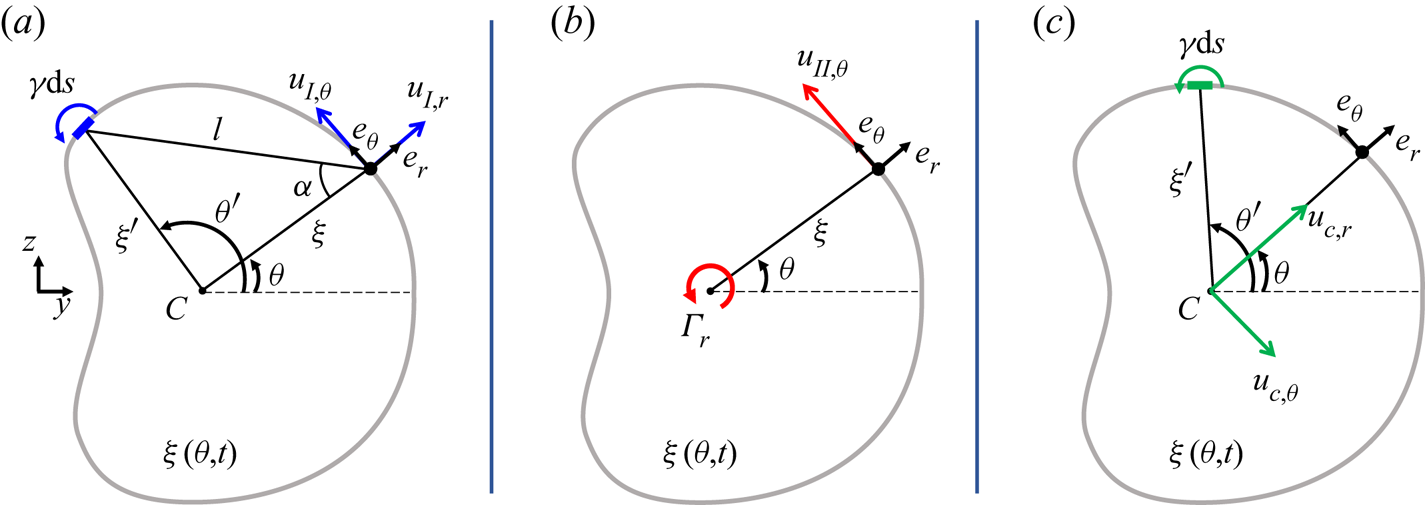
\includegraphics[width=12cm]{fig1.png}  %需调整
    \caption{面涡上不同速度分量的示意图}
\end{figure}

接下来设面涡强度有:$\gamma =\gamma (\theta,t)$,则可以给出
面涡的自诱导速度。除了面涡的自诱导,在点$C$处还有一个
$\varGamma_r$环量的点涡。
设其初始条件是:
\begin{gather} \gamma_0=\gamma(\theta,0)=\gamma_r+\gamma_b\sin\theta \quad \textrm{at}\ r=\xi_0, \end{gather}
\begin{gather}\varGamma_r={-}2{\rm \pi}\xi\gamma_r \quad\textrm{at } r=0, \end{gather}
初始条件中$\gamma_b$是由于偏航造成的。$\gamma_b,\gamma_r$都是和
风机工况相关的常数。

面涡的运动速度,相对于$C$点来说是:
\begin{equation} \underbrace{\boldsymbol{u}(\theta,t)}_{\substack{\text{vortex sheet velocity} \\ \text{with respect to C}}}=\underbrace{\boldsymbol{u}_{I}}_{\substack{\text{self-induced} \\ \text{vortex sheet velocity}}}+\underbrace{\boldsymbol{u}_{II}}_{\substack{\text{vortex sheet velocity induced} \\ \text{by point vortex at C}}}-\underbrace{\boldsymbol{u}_{c}}_{\substack{\text{velocity} \\ \text{of C}}}. \end{equation}

根据毕奥-萨伐尔定律可以给出自诱导速度为:
\begin{gather} u_{I,r}(\theta,t)=\int_0^{2{\rm \pi}}\frac{\gamma(\theta',t)\sin{\alpha}}{2{\rm \pi} l}\xi'\,\textrm{d}\theta', \end{gather}
\begin{gather}u_{I,\theta}(\theta,t)=\int_0^{2{\rm \pi}}\frac{\gamma(\theta',t)\cos{\alpha}}{2{\rm \pi} l}\xi'\,\textrm{d}\theta', \end{gather}
其中几何量的定义可见示意图。

文章根据三角代数关系化简得到:
\begin{gather} u_{I,r} (\theta,t) = {p.v.}\frac{1}{4{\rm \pi}} \int_{0}^{2{\rm \pi}} \frac{\gamma(\theta',t)}{\tan{\left[\left(\theta'-\theta\right)/2\right]}}\textrm{d}\theta', \end{gather}
\begin{gather}u_{{I}, \theta} (\theta,t) = {p.v.}\frac{1}{4{\rm \pi}}\int_{0}^{2{\rm \pi}} \frac{\gamma(\theta',t)\sin{\left[\left(\theta'-\theta\right)/2\right]}}{\sin{\left[\left(\theta'-\theta\right)/2\right]}}\textrm{d}\theta'= \frac{1}{4{\rm \pi}}\int_{0}^{2{\rm \pi}}\gamma(\theta')\,\textrm{d}\theta'. \end{gather}
以上积分中,$p.v.$指的是积分取柯西主值,因为存在不收敛的奇点积分。

点涡对涡面的诱导速度比较容易得到:
\begin{gather} u_{{II},r} (\theta,t) = 0, \end{gather}
\begin{gather}u_{{II},\theta} (\theta,t) = \frac{\varGamma_r}{2{\rm \pi} \xi}={-}\gamma_r. \end{gather}

面涡对点涡的诱导速度构成了$C$的速度,构成了面涡上面一点的牵连速度:
\begin{gather} u_{c,r}(\theta,t)=\frac{1}{2{\rm \pi}}\int_0^{2{\rm \pi}}\gamma(\theta',t) \sin\left({\theta'-\theta}\right)\textrm{d}\theta', \end{gather}
\begin{gather}u_{c,\theta}(\theta,t)={-}\frac{1}{2{\rm \pi}}\int_0^{2{\rm \pi}}\gamma(\theta',t) \cos\left({\theta'-\theta}\right)\textrm{d}\theta'. \end{gather}

忽略流向的拉伸,则面涡强度是守恒的,有输运方程:
\begin{equation} \frac{\partial \gamma}{\partial t}+ \frac{\partial\left(\gamma u_s\right)}{\partial s}=0, \end{equation}

当时间较小且偏航较小时,面涡接近圆形,上式可以近似为:
\begin{equation} \frac{\partial \gamma}{\partial t}+ \frac{1}{\xi}\frac{\partial (\gamma u_\theta)}{\partial \theta}\approx 0. \end{equation}

用$\gamma_b,\xi_0$对方程无量纲化,则有:
\begin{gather}\label{eq:evUR} \hat{u}_{r}(\theta,\hat{t})\approx {p.v.}\frac{1}{4{\rm \pi}} \int_{0}^{2{\rm \pi}} \frac{\hat{\gamma}(\theta',\hat{t})}{\tan{\left[\left(\theta'-\theta\right)/2\right]}}\textrm{d}\theta' -\frac{1}{2{\rm \pi}}\int_0^{2{\rm \pi}}\hat{\gamma}(\theta',\hat{t})\sin\left({\theta'-\theta}\right)\textrm{d}\theta', \end{gather}
\begin{gather}\label{eq:evUT}\hat{u}_{\theta}(\theta,\hat{t})\approx\frac{1}{4{\rm \pi}} \int_{0}^{2{\rm \pi}}\hat{\gamma}(\theta')\,\textrm{d}\theta'+\frac{1}{2{\rm \pi}} \int_0^{2{\rm \pi}}\hat{\gamma}(\theta',\hat{t})\cos\left({\theta'-\theta}\right)\textrm{d}\theta'-\chi, \end{gather}
\begin{gather}\label{eq:evGM}\frac{\partial \hat{\gamma}}{\partial \hat{t}} \approx{-}\frac{1}{\hat{\xi}} \frac{\partial (\hat{\gamma} \hat{u}_\theta)}{\partial \theta}. \end{gather}


\section{幂级数近似的解析解}

将自变量写成时间方向的幂级数形式,则有:
\begin{equation} \hat{\gamma}(\theta,\hat{t}) = \sum _{n=0}^{\infty} \hat{\gamma}_{n}(\theta)\hat{t}^{n}; \quad \hat{u}_r(\theta,\hat{t}) = \sum _{n=0}^{\infty} \hat{u}_{r n}(\theta)\hat{t}^{n}, \quad \hat{u}_{\theta}(\theta,\hat{t}) =\sum _{n=0}^{\infty} \hat{u}_{\theta n}(\theta)\hat{t}^{n}. \end{equation}

则面涡形状展开为:
\begin{gather} \hat{\xi}=1+\int \hat{u}_r\,\textrm{d}\hat{t}=1+\sum _{n=0}^{\infty} \frac{1}{n+1} \hat{u}_{r n} \hat{t}^{n+1}, \end{gather}
\begin{gather}\frac{1}{\hat{\xi}} = \sum _{n=0}^{\infty} f_{n}(\theta)\hat{t}^{n}, \end{gather}
其中$f_n$是$\frac{1}{\hat{\xi}}$的幂级数系数。

将幂级数代入速度和涡强表达式可得:
\begin{gather}\label{eq:A} \hat{u}_{rn}(\theta)\approx {p.v.}\frac{1}{4{\rm \pi}} \int_{0}^{2{\rm \pi}} \frac{\hat{\gamma}_n(\theta')}{\tan{\left[\left(\theta'-\theta\right)/2\right]}}\textrm{d}\theta' -\frac{1}{2{\rm \pi}}\int_0^{2{\rm \pi}}\hat{\gamma}_n(\theta')\sin\left({\theta'-\theta}\right)\textrm{d}\theta', \end{gather}
\begin{gather}\label{eq:B} \hat{u}_{\theta n}(\theta)\approx\frac{1}{4{\rm \pi}} \int_{0}^{2{\rm \pi}}\hat{\gamma}_n(\theta')\,\textrm{d}\theta'+\frac{1}{2{\rm \pi}} \int_0^{2{\rm \pi}}\hat{\gamma}_n(\theta')\cos\left({\theta'-\theta}\right)\textrm{d}\theta'- \begin{cases} \chi, & \text{if } n=0, \\ 0, & \text{if } n>0, \end{cases} \end{gather}
\begin{gather}\label{eq:C} \hat{\gamma}_{n+1} \approx{-}\frac{1}{(n+1)} \left(\sum_{j=0}^{n}f_{j} \sum_{i=0}^{n-j} \frac{\partial (\hat{\gamma}_i \hat{u}_{\theta (n-j-i)})}{\partial \theta}\right). \end{gather}

本文给出了主值积分:
\begin{gather} {p.v.} \int_{0}^{2{\rm \pi}} \frac{\sin{n x}}{\tan{\left[\left(x-b\right)/2\right]}}\textrm{d}\kern0.06em x=2{\rm \pi}\cos{nb}, \end{gather}
\begin{gather}{p.v.} \int_{0}^{2{\rm \pi}} \frac{\cos mx}{\tan{\left[\left(x-b\right)/2\right]}}\textrm{d}\kern0.06em x={-}2{\rm \pi}\sin{mb}. \end{gather}
用于化简。

初始条件可得$\hat {\gamma }_0(\theta )=\sin \theta +\chi$,因此
代入\eqref{eq:A}\eqref{eq:B}可得面涡运动速度的零阶项$\hat {u}_{r0}(\theta ),\hat {u}_{\theta 0}(\theta )$。
将零阶项的速度代入\eqref{eq:C}可得一阶项的涡强。
这样递归地代入,即可得到幂级数展开中的任意阶项,达到任意阶逼近精度。
随后安装时间积分则有面涡形状的逼近。
本文将$\hat {\gamma }, \hat{u}_r, \hat{u}_\theta$展开到${O}(\hat {t}^{3})$,
$\hat {\xi }$为${O}(\hat {t}^{4})$时,有级数解:

\begin{align} \hat{\gamma}(\theta,\hat{t}) &= \sin (\theta ) + \chi -\frac{1}{2} \hat{t} \sin (2 \theta ) +\hat{t}^{2} \left(-\frac{1}{4} \chi \cos (2 \theta )+\frac{3}{16} \sin (3 \theta )-\frac{\sin (\theta )}{16}\right) \nonumber\\ &\quad +\hat{t}^{3} \left(\frac{1}{12} \chi ^{2} \sin (2 \theta )-\frac{1}{48} \chi \cos (\theta )+\frac{5}{32} \chi \cos (3 \theta ) \right.\nonumber\\ &\quad \left.+\frac{5}{96} \sin (2\theta )-\frac{7}{96} \sin (4 \theta )\right),  \end{align}
\begin{align} \hat{u}_r(\theta,\hat{t}) &={-}\frac{1}{4} \hat{t} \cos (2 \theta )+ \hat{t}^{2} \left(\frac{1}{8} \chi \sin (2 \theta )+\frac{3}{32} \cos (3 \theta )\right) \nonumber\\ &\quad + \hat{t}^{3} \left(\frac{1}{24} \chi ^{2} \cos (2 \theta )-\frac{5}{64} \chi \sin (3 \theta )+\frac{5}{192} \cos (2 \theta )-\frac{7}{192} \cos (4 \theta )\right),  \end{align}
\begin{align} &\qquad\ \hat{u}_{\theta}(\theta,\hat{t}) = \frac{1}{2}\sin (\theta ) - \frac{1 }{2}\chi -\frac{1}{32} \hat{t}^{2} \sin (\theta ) -\frac{1}{96} \hat{t}^{3} \chi \cos (\theta ), \end{align}
\begin{align} \hat{\xi}(\theta,\hat{t}) &= 1 -\frac{1}{8} \hat{t}^{2} \cos (2 \theta )+\hat{t}^{3} \left(\frac{1}{24} \chi \sin (2 \theta )+\frac{1}{32} \cos (3 \theta )\right)\nonumber\\ &\quad +\hat{t}^{4} \left(\frac{1}{96} \chi ^{2} \cos (2 \theta)-\frac{5}{256} \chi \sin (3 \theta )+\frac{5}{768} \cos (2 \theta)-\frac{7}{768} \cos (4 \theta )\right). \end{align}

事实上,由于级数逼近,以上的解只在时间很短,如$|\hat {t}|\leq2$的意义下
成立。本文在附录中给出了在时间较大时预测面涡的一种经验公式,
其在时间较小时退化到以上的幂级数解析解。

本文还专门对于初始条件中的各种参数,给出了其在具体风机
工况下的计算方法。在阅读报告不再赘述。

\section{面涡横向偏移}

接下来本文给出了尾迹面涡的横向轨迹偏移。
由于以上给出的面涡时间演化是在中心涡的坐标系下的,
还需要给出中心的偏移轨迹。
时间积分可得:
\begin{gather} \hat{y}_c=\frac{\hat{t}}{2}-\frac{\hat{t}^{3}}{96}, \end{gather}
\begin{gather}\hat{z}_c=\frac{\chi\hat{t}^{4}}{384}. \end{gather}

在时间较长时,上式的误差较大,因为此时尾迹已经
接近卷成一个双涡结构(CVP),与圆形偏差较大。
因此,本文根据CVP结构给出时间较长时的轨迹。
根据B-S定律:
\begin{equation} v_c=\frac{2\varGamma_b}{2{\rm \pi} L}\cos\alpha=\frac{\varGamma_b \xi_0}{{\rm \pi} \left(\xi_0^{2}+\delta_c^{2}\right)}, \end{equation}
上式是根据示意图中CVP的结构给出的。
涡对的自诱导给出:
\begin{equation} \frac{\textrm{d}\delta_c}{\textrm{d}t}=v_c-v_{cvp}= \frac{\varGamma_b \xi_0}{{\rm \pi} \left(\xi_0^{2}+\delta_c^{2}\right)}- \frac{\varGamma_b}{4{\rm \pi}\xi_0}=\frac{\varGamma_b}{4{\rm \pi} \xi_0} \left(\frac{3\xi_0^{2}-\delta_c^{2}}{\xi_0^{2}+\delta_c^{2}}\right). \end{equation}

近似$\varGamma _b \approx 2\xi _0\gamma _b$可积分得到:
\begin{equation} \frac{\hat{t}}{2{\rm \pi}}=\frac{-2}{\sqrt{3}}\ln{\left(\frac{\sqrt{3}-\hat{\delta}_c}{\sqrt{3}+ \hat{\delta}_c}\right)}-\hat{\delta}_c, \end{equation}
因此
\begin{equation} \hat{y}_c=\hat{\delta}_c +\frac{\hat{t}}{2{\rm \pi}}. \end{equation}

本文通过类似Pade逼近的思路,给出经验公式,使得其
在小时间时趋近于面涡精确解而大时间时趋近于CVP的尾涡精确解:
\begin{equation} \label{eq:emp}\hat{y}_c=\frac{({\rm \pi}-1)|\hat{t}|^{3}+2\sqrt{3}{\rm \pi}^{2}\hat{t}^{2}+48({\rm \pi}-1)^{2} |\hat{t}|}{2{\rm \pi}({\rm \pi}-1)\hat{t}^{2}+4\sqrt{3}{\rm \pi}^{2}|\hat{t}|+96({\rm \pi}-1)^{2}}\textrm{sgn}(\hat{t}). \end{equation}


\begin{figure}[H]
    \centering
    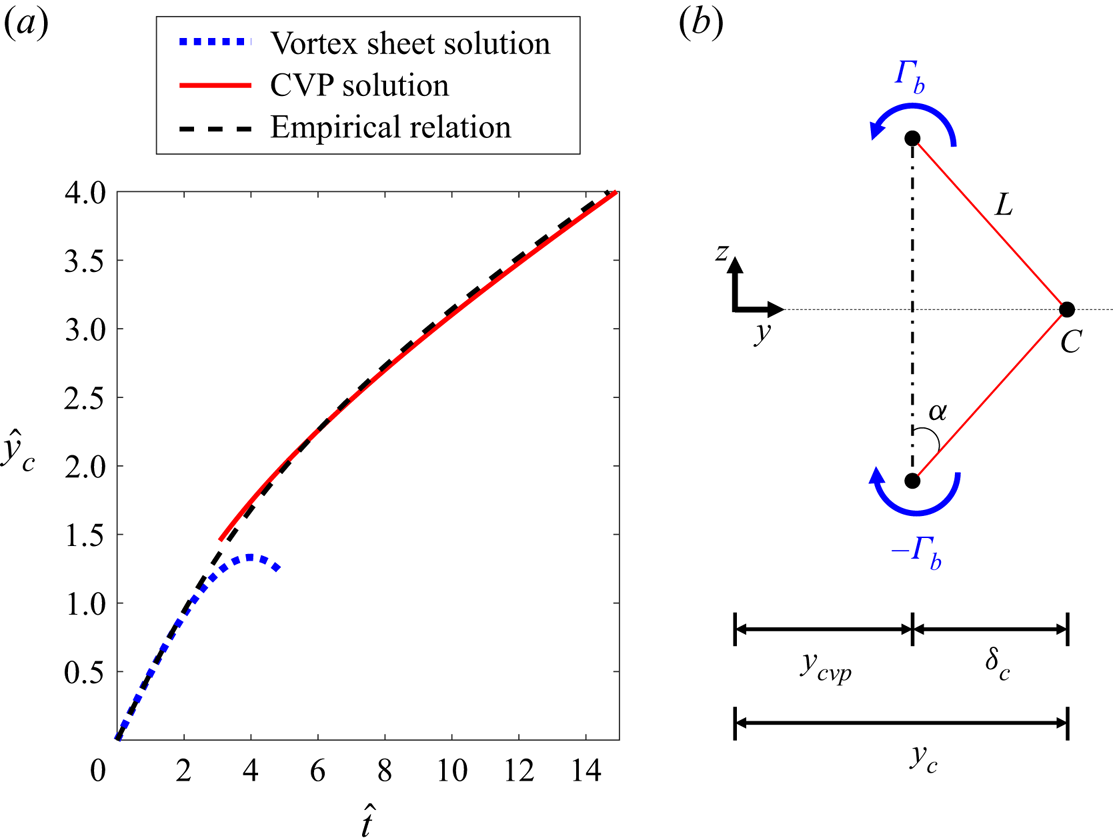
\includegraphics[width=12cm]{Fig4.png}  %需调整
    \caption{涡心轨迹解对比与CVP几何示意}
\end{figure}

上图给出了不同的解的对比。

\section{与数值模拟的对比}

本文采用LES计算程序LESGO进行对比,
风机是旋转器作动盘模型(ADM-R),
计算中来流是均匀的,
因此大部分时候实际上是无粘的计算。
更多计算细节详见原文。

为了对比尾迹解析模型的精确程度,
给出用于代入解析模型的参数:
$\hat {t}=\gamma _bt/\xi _0$,$t=x/U_{con}$,
其中对流速度$U_{con}$当作常数,虽然
下游的对流速度有一定变化。
在无粘计算中,由于掺混很小,
尾迹中央可以认为是均匀速度$U_0 = U_{{in}}\sqrt {1-C_T\cos ^{2}\beta }$,
来流为$U_{in}$,那么对流速度按照$U_{con} = 0.5(U_0 + U_{in})$计算。
这是无粘算例中较为常用的作法。
同时,数值解中尾迹的边缘按照流管给出,流管的初始位置是作动盘的边缘。

\begin{figure}[H]
    \centering
    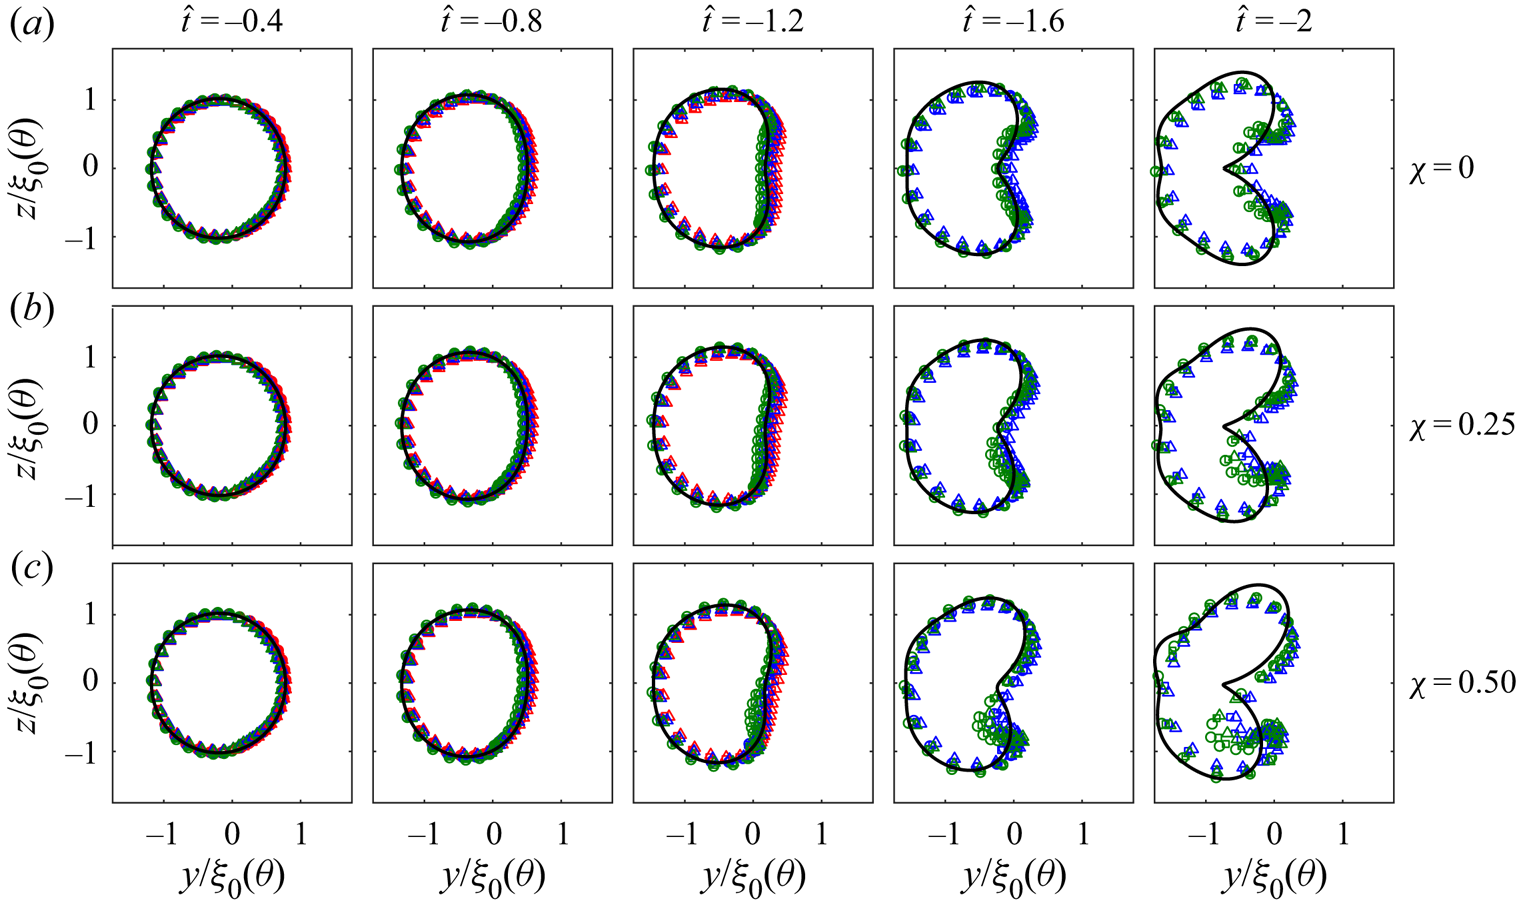
\includegraphics[width=12cm]{Fig5.png}  %需调整
    \caption{无量纲尾迹的对比,其中黑线是解析解,符号是不同推力系数的数值解}
\end{figure}

上图给出无量纲化后尾迹形状的对比,可见不同算例无量纲化后尾迹确实可以接近重合;
尾迹形状在不同时间和旋转律都与解析解基本吻合。
时间较大后,变形很大,因此差别较大。

\begin{figure}[H]
    \centering
    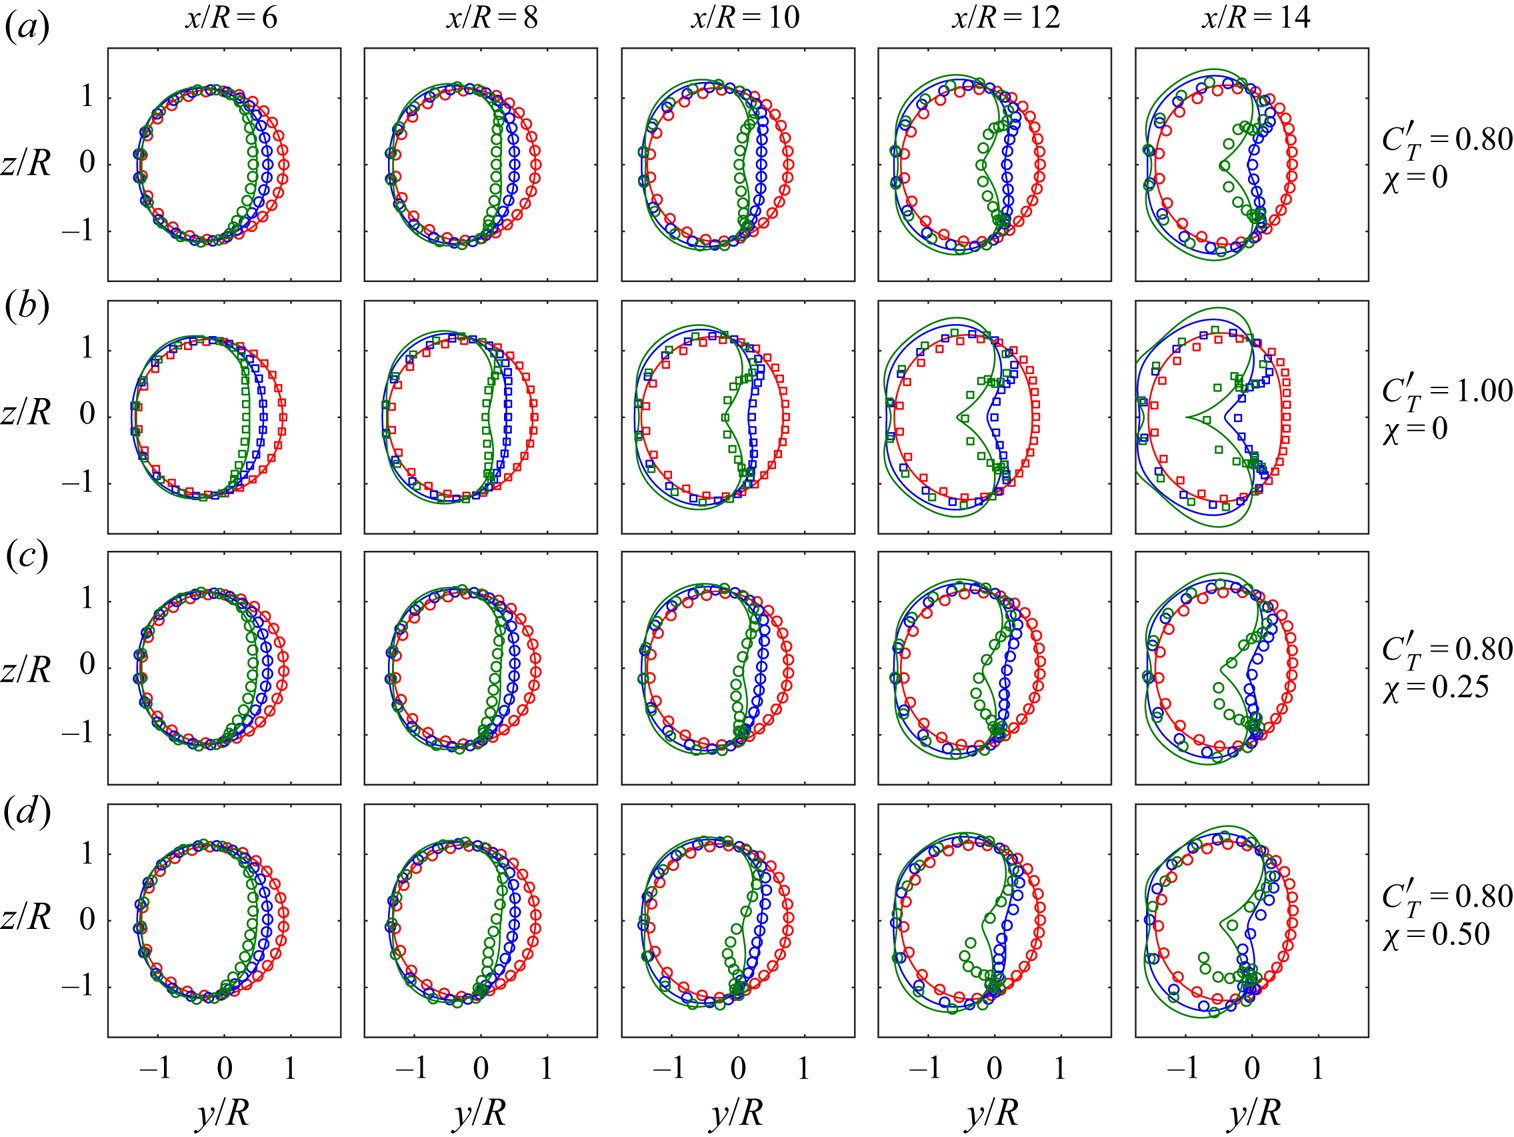
\includegraphics[width=12cm]{Fig6.png}  %需调整
    \caption{物理坐标尾迹的对比,其中实线是解析解,符号是数值解,不同颜色是不同偏航角}
\end{figure}

上图是有量纲尾迹形状的对比,可见在较小偏航角、较短时间时,
尾迹的预测较为准确,否则与数值结果吻合变差。

\section{湍流大气边界中的面涡演化}

以上的推导是基于无粘流动的,因此涡强度不会衰减。
在湍流大气边界中还需要考虑湍流的影响。

根据文章,设$\gamma_b,\gamma_r$是时间的函数,并且:
\begin{equation} \gamma(\theta,t) = \gamma_b(t) \hat{\gamma}(\theta,\hat{t}),\quad {u}_r(\theta,t)= \gamma_b(t)\hat{u}_r(\theta,\hat{t}),\quad {u}_{\theta}(\theta,t)=\gamma_b(t) \hat{u}_{\theta}(\theta,\hat{t}). \end{equation}
同时将位移和时间缩放:
\begin{gather} \hat{\xi}(\theta,\hat{t})=\frac{\xi(\theta,t)}{\xi_0}, \end{gather}
\begin{gather}\hat{t}(t)=\frac{1}{\xi_0}\int_0^{t}\gamma_b(t')\,\textrm{d}t', \end{gather}
可以保持\eqref{eq:evUR}\eqref{eq:evUT}\eqref{eq:emp}的形式
不变;但是\eqref{eq:evGM}变成了:
\begin{equation} \frac{\partial \hat{\gamma}}{\partial \hat{t}}+\frac{1}{\hat{\xi}} \frac{\partial (\hat{\gamma} \hat{u}_\theta)}{\partial \theta}\approx{-} \frac{\xi_0\hat{\gamma}}{\gamma^{2}_b}\frac{\textrm{d} \gamma_b}{\textrm{d} t}. \end{equation}

考虑边界层的速度分布,近似认为:$U_{con}=U_{{in}}(z)$,$t \approx x/U_{{in}}(z)$。

本文直接采用了一个Shaprio的环量衰减模型:
\begin{equation} \frac{\varGamma_b(x)}{\varGamma_{b0}}=\frac{\sqrt{\rm \pi}}{4}\frac{R}{\eta(x)} \exp\left(-\frac{R^{2}}{8\eta^{2}(x)}\right)\left[I_0\left(\frac{R^{2}}{8\eta^{2}(x)}\right)+I_1 \left(\frac{R^{2}}{8\eta^{2}(x)}\right)\right], \end{equation}

因此可积分处湍流修正过的无量纲时间:
\begin{equation} \hat{t}=\frac{24^{1/4}}{2k_{\nu}U_{{in}}(z)\xi_0 R }\int_0^{\eta}\varGamma_b(\eta')\,\textrm{d}\eta'. \end{equation}
将其中环量的变化用拟合式替换,则有:
\begin{equation} \hat{t}(x,z)\approx{-}1.44 \frac{U_h}{u_*}\frac{R}{\tilde{\xi}_0} C_T \cos^{2}\beta \sin\beta \left[1-\textrm{exp}\left({-}0.35\frac{u_*}{U_\textrm{in}(z)}\frac{x}{R}\right)\right]. \end{equation}
是无量纲时间的计算公式。

\begin{figure}[H]
    \centering
    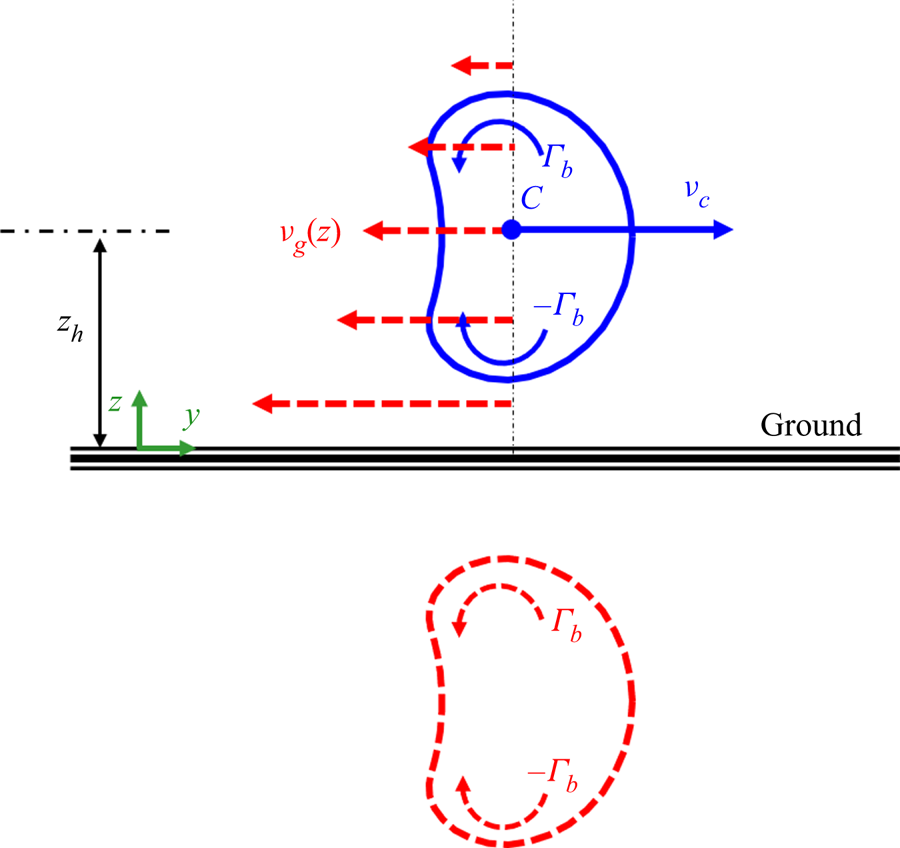
\includegraphics[width=12cm]{Fig7.png}  %需调整
    \caption{镜像面涡示意}
\end{figure}

为了模拟地面效应,本文采用了一个镜像面涡近似,如上图,这样
尾迹的诱导速度不影响壁面边界。按照CVP近似涡面,
则镜像CVP的诱导速度:
\begin{equation} v_g=\frac{\varGamma_b}{2{\rm \pi}} \left[\frac{1}{z+z_h-\xi_0} -\frac{1}{z+z_h+\xi_0}\right] = \frac{\varGamma_b \xi_0}{{\rm \pi}\left[(z+z_h)^{2}-\xi_0^{2}\right]}. \end{equation}
由于地面造成的横向位移:
\begin{equation} y_g(z) = \int_0^{t} v_g(z,t') \,\textrm{d} t' = \frac{\xi_0 \displaystyle\int_0^{t} \varGamma_b(t') \,\textrm{d} t}{{\rm \pi} \left[(z+z_h)^{2}-\xi_0^{2}\right]}. \end{equation}
近似$\varGamma _b \approx 2\xi _0\gamma _b$,
并且使用$\hat {t} = \int _0^{t} \gamma _b(t') / \xi _0 \,\textrm {d} t'$,
则有:
\begin{equation} \hat{y}_g = \frac{2}{\rm \pi} \frac{\hat{t}}{\left[ {(z+z_h)}/{\xi_0}\right]^{2}-1}, \end{equation}
进一步有考虑地面效应的涡心运动轨迹:
\begin{equation} \hat{y}_c = \frac{({\rm \pi}-1)|\hat{t}|^{3}+2\sqrt{3}{\rm \pi}^{2}\hat{t}^{2}+48 ({\rm \pi}-1)^{2}|\hat{t}|}{2{\rm \pi}({\rm \pi}-1)\hat{t}^{2}+4\sqrt{3}{\rm \pi}^{2}|\hat{t}|+96({\rm \pi}-1)^{2}} \textrm{sgn}(\hat{t}) - \frac{2}{\rm \pi}\frac{\hat{t}}{[({z+z_h})/{\tilde{\xi}_0}]^{2}-1}. \end{equation}

基于以上尾迹形状预测的模型,
本文进一步推导了关于尾迹速度分布的解析模型。尾迹速度分布的推导
思路是,将圆形尾迹的Gaussian速度分布模型修正以应用于以上给出的卷起的尾迹形状。
文章还总结了预测湍流尾迹的步骤:(1)计算初始尾迹形状的近似;(2)计算无量纲时间;(3)计算涡心位置;
(4)计算极坐标角度;(5)计算初始尾迹形状分布;(6)计算不同时间的尾迹形状;
(7)根据湍流尾迹速度分布计算尾迹宽度;(8)计算湍流尾迹最大速度损失;(9)计算尾迹速度损失的分布。

文章将上述预测结果与LES湍流结果以及实验对比,发现解析模型可以较好预测
尾迹速度分布,并且较好估算尾迹中下游风机的功率,结果与LES相仿。

\section{总结}

本文发展了一系列解析模型,用于预测均匀和湍流来流情况下偏航风机的
尾迹形状以及速度分布。本文首先按照给出了理想面涡附加点涡形式的
尾迹初值,并且按照平面涡运动的诱导速度关系给出了面涡的
运动规律。本文按照幂级数方法求解了运动方程,给出了面涡形状的解析公式,
和涡心偏移位置的解析公式,适用于较小时间。
接下来本文
推导了涡面形状和尾迹位置的经验公式,用于在更大时间较好吻合实际情况
同时在较小时间与解析解吻合。
从无粘模型出发,本文进一步将其修正为湍流情况的尾迹形状,
并且给出了一个尾迹速度分布的模型。
本文的解析模型与数值模拟都有较好的吻合,表明
本文的模型模拟了偏航风机尾迹流动中最主要的流体力学效应。
本文的模型相对于数值模拟计算量很小,对于风机的风场控制和优化
过程有一定帮助。


\section{体会和思考}
本文推导的出发点就是基于面涡的二维运动,
其控制方程为面涡自诱导运动与点涡诱导速度等,
具有理论上的简洁性。同时,为了求解非线性的运动方程
本文首先对求解的时间范围进行限制,来对求解的几何进行简化。
经过简化之后,本文给出了幂级数形式的求解步骤,
计算了幂级数形式的面涡运动近似解。
可见,理想模型与近似条件在得到简单形式的表达式的过程中是不可或缺的。

当然,推出简单表达式后并不意味着一定适用。本文就在时间
较大后换成其他模型,如涡对CVP结构来近似,弥补
面涡模型不适用的范围。
同时,在湍流条件下需要具体修正才能使用面涡模型的结果。

另外一方面,本文最后适用于湍流大气边界的结果具有一定工程价值,
但是直接构思适用于湍流的尾迹模型其实很困难。因此,本文的思路基本上是,
先推导一个无粘情况的模型,随后用合理的方式将其修正,
得到很成功的湍流情况的模型。
这说明,在尾迹中,湍流平均运动的许多特性,
基本和无粘情况一致,或许只需在某些方面加入关于湍流耗散
和不均匀平均速度的影响,就可以与实际情况很好吻合。

阅读本文最深的感受是,如果能够找到合适的理想模型,
经过简化之后可以将其近似求解,也可以在一定情况下
得到近似程度很高的理论模型。这种思路,在飞行器设计中
就类似边界层积分加势流的结合,可以很好预测
大部分飞机部件的主要升阻力特性,在工程实践中可以应用于快速选型等。
这种模型的提出过程,就需要对流动特征有很好的物理直觉,
能够抓住主要的流动结构,
并且能够根据流动特征进行有效的简化而不是
困在难以求解的未简化模型中。

本文的思路下,另一种方法是搭建一种近似的数值方法,利用
尾迹的二维简化的特性,在平面内数值求解涡运动方程,
这样尾迹速度分布的计算量也很小(相对于LES),并且可能在极端条件下结果更可靠。
另外,本文的模型还可以进一步改进考虑地面效应的影响,考虑
面涡形状受到地面的影响而非只考虑其横向位置的变化。
同时,对于更复杂湍流来流条件和非定常来流条件怎样计算也可以进一步考虑研究。


\bibliography{refs}{}
\bibliographystyle{unsrt}

% \section*{附录}
% 本文计算代码都在\href{https://github.com/harryzhou2000/HW_ACFD}{Github Repo中(点击访问)}。































% \section{SECTION 节}

% 一个

% \subsection{SUBSECTION 小节}

% 示例

% \subsubsection{SUBSUBSECTION 小节节}

% 字体字号临时调整:
% {
%    \sffamily\bfseries\zihao{3} 哈哈哈哈哈 abcde %三号 sans系列字体(一开始设置的) 加粗
%    %只对大括号范围内的后面的字有用,在标题、题注里面同样
% }
% { 
%    \CJKfamily{kaiti}\zihao{5}\itshape 哈哈哈哈哈 abcde%三号 kaiti(一开始设置的, 斜体(英文有变)
%    %只对大括号范围内的后面的字有用,在标题、题注里面同样
% }

% 一大堆一大堆一大堆一大堆一大堆一大堆一大堆一大堆一大堆一大堆
% 一大堆一大堆一大堆一大堆一大堆一大堆一大堆一大堆一大堆一大堆一大堆一大堆
% 一大堆一大堆一大堆一大堆一大堆一大堆一大堆一大堆一大堆一大堆一大堆一大堆
% 一大堆一大堆一大堆一大堆一大堆一大堆一大堆一大堆一大堆一大堆一大堆一大堆

% \begin{center}
%     居中的什么乱七八糟东西
% \end{center}


% 一个列表:
% \begin{itemize}
%     \item asef
%     \item[\%] asdf
%     \item[\#] aaa
% \end{itemize}

% 一个有序列表:
% \begin{enumerate}
%     \item asef
%     \item[\%\%] asdf
%     \item aaa
% \end{enumerate}

% 一个嵌套列表,考虑缩进:
% \begin{enumerate}[itemindent=2em] %缩进
%     \item asef \par asaf 东西东西东西东西东西东西东西东西东西东西东西东西东西东西东西东西东西东西东西东西东西东西东西东西,
%           F不是不是不是不是不是不是不是不是不是不是不是不是不是不是不是
%           \begin{itemize}[itemindent=2em]  %缩进
%               \item lalala
%               \item mamama
%           \end{itemize}
%     \item asdf
%     \item aaa
% \end{enumerate}

% \section{SECTION}

% 图片排版:

% \begin{figure}[H]
%     \begin{minipage}[c]{0.45\linewidth}  %需调整
%         \centering
%         \includegraphics[width=8cm]{RAM_O2_4660.png}  %需调整
%         \caption{第一个图}
%         \label{fig:a}
%     \end{minipage}
%     \hfill %弹性长度
%     \begin{minipage}[c]{0.45\linewidth}  %需调整
%         \centering
%         \includegraphics[width=8cm]{RAM_O4_4660.png}  %需调整
%         \caption{第二个图}
%         \label{fig:b}
%     \end{minipage}
% \end{figure}

% figure的选项为“htbp”时,会自动浮动,是“H”则和文字顺序严格一些。

% \begin{figure}[H]
%     \begin{minipage}[c]{0.45\linewidth}  %需调整
%         \centering
%         \includegraphics[width=8cm]{RAM_O2_4660.png}  %需调整
%         \label{fig:x}
%     \end{minipage}
%     \hfill %弹性长度
%     \begin{minipage}[c]{0.45\linewidth}  %需调整
%         \centering
%         \includegraphics[width=8cm]{RAM_O4_4660.png}  %需调整
%         \label{fig:y}
%     \end{minipage}
%     \caption{第三个图}
% \end{figure}

% \begin{figure}[H]
%     \centering
%     \includegraphics[width=8cm]{RAM_O4_4660.png}  %需调整
%     \label{fig:c}
%     \caption{第四个图}
% \end{figure}



% \subsection{SUBSECTION}

% 关于怎么搞表格:

% \begin{table*}[htbp]
%     \footnotesize
%     \begin{center}
%         \caption{一端力矩载荷下的结果\fontsize{0pt}{2em}} %需要学习统一设置;0代表不变?
%         \label{表2}
%         \begin{tabular}{|c|c|c|c|c|c|c|}
%             \hline
%             节点数                              & 积分方案              & 单元数                & $h=1m$                & $h=0.1m$              & $h=0.05m$             & $h=0.01m$             \\
%             \hline
%             \multirow{6}{*}{2}                  & \multirow{3}{*}{精确} & 1                     & 4.235294117647059E-08 & 1.406250000000000E-06 & 2.862823061630218E-06 & 1.439654482924097E-05 \\
%             \cline{3-7}
%                                                 &                       & 10                    & 5.975103734439814E-08 & 4.235294117646719E-05 & 1.800000000000410E-04 & 1.406249999999849E-03 \\
%             \cline{3-7}
%                                                 &                       &
%             10000                               & 5.999999915514277E-08 & 5.999996622448291E-05 & 4.799989509752562E-04 & 5.999793702477535E-02                                                 \\
%             \cline{2-7}
%                                                 & \multirow{3}{*}{减缩} & 1                     & 6.000000000000001E-08 & 5.999999999999972E-05 & 4.799999999999911E-04 & 6.000000000003492E-02 \\
%             \cline{3-7}
%                                                 &                       & 10                    & 6.000000000000071E-08 & 5.999999999999142E-05 & 4.799999999995399E-04 & 5.999999999903294E-02 \\
%             \cline{3-7}
%                                                 &                       & 10000                 & 6.000000112649221E-08 & 5.999999234537814E-05 & 4.799997501925065E-04 & 6.000037607984510E-02 \\
%             \hline

%             \multirow{6}{*}{3}                  & \multirow{3}{*}{精确} & 1                     & 6.000000000000003E-08 & 6.000000000000202E-05 & 4.800000000000831E-04 & 6.000000000056749E-02 \\
%             \cline{3-7}
%                                                 &                       & 10                    & 5.999999999999932E-08 & 6.000000000004190E-05 & 4.800000000000206E-04 & 6.000000001613761E-02 \\
%             \cline{3-7}
%                                                 &                       & 10000                 & 6.000000013769874E-08 & 5.999989495410481E-05 & 4.799942099727246E-04 & 6.000263852944890E-02 \\
%             \cline{2-7}
%                                                 & \multirow{3}{*}{减缩} & 1                     & 6.000000000000002E-08 & 6.000000000000267E-05 & 4.800000000000754E-04 & 5.999999999989982E-02 \\
%             \cline{3-7}
%                                                 &                       & 10                    & 5.999999999999899E-08 & 5.999999999987338E-05 & 4.799999999947916E-04 & 5.999999998625345E-02 \\
%             \cline{3-7}
%                                                 &                       & 10000                 & 5.999999728157785E-08 & 5.999994914321980E-05 & 4.800008377474699E-04 & 5.999472246346305E-02 \\
%             \hline

%             \multicolumn{3}{|c|}{欧拉-伯努利解} & 6.000000000000000E-08 & 6.000000000000000E-05 & 4.800000000000000E-04 & 6.000000000000000E-02                                                 \\
%             \hline
%         \end{tabular}
%     \end{center}
% \end{table*}

% 多行、多列表格的示例,基本思想是,多列的那个东西放在多列的最上面一格,下面的行要用\&来空开,也就是\&的数目
% 和普通表格一样,是列数减一;
% 多列的部分的话,就是每行内的操作,相应的\&就少了,见最后一行。

% tabular的“|c|c|c|c|c|c|c|”,意思是,竖线-居中-竖线-居中-竖线……,可以选择省略一些竖线;
% 每行之间的hline,代表贯通的横线,cline是有范围的横线。

% \subsubsection{SUBSUBSECTION}

% newcommand可以用来定义新指令,似乎基本上就是字符串替换……不太懂,总之在公式里面可以用,
% 外面也经常用。






% 公式这么写:
% \begin{equation}
%     \begin{aligned}
%         \frac{aa(x^1+x^2)}{\sqrt{x^1x^2}}
%         \nabla\times\uu
%         = & u_{j;m}\g^m\times\g^j
%         =u_{j;m}\epsilon^{mjk}\g_k
%         =u_{j,m}\epsilon^{mjk}\g_k                           \\
%         = & \frac{1}{\sqrt{g}}\left|
%         \begin{matrix}
%             \g_1       & \g_2       & \g_3       \\
%             \partial_1 & \partial_2 & \partial_3 \\
%             u_1        & u_2        & u_3
%         \end{matrix}
%         \right|
%         =\frac{\sqrt{x^1x^2}}{aa(x^1+x^2)}
%         \left|
%         \begin{matrix}
%             \g_1                        & \g_2                        & \g_3       \\
%             \partial_1                  & \partial_2                  & \partial_3 \\
%             u^1\frac{a^2(x^1+x^2)}{x^1} & u^2\frac{a^2(x^1+x^2)}{x^2} & u^3
%         \end{matrix}
%         \right|                                              \\
%         = & \frac{\sqrt{x^1x^2}}{aa(x^1+x^2)}
%         [[\g_1\,\g_2\,\g_3]]
%         diag\left(
%         u^3_{,2}-u^2_{,3}\frac{a^2(x^1+x^2)}{x^2},\,
%         u^1_{,3}\frac{a^2(x^1+x^2)}{x^1}-u^3_{,1},\, \right. \\
%           & \left.
%         u^2_{,1}\frac{a^2(x^1+x^2)}{x^2}+u^2\frac{a^2}{x^2}
%         -
%         u^1_{,2}\frac{a^2(x^1+x^2)}{x^1}-u^1\frac{a^2}{x^1}
%         \right)                                              \\
%         = & \frac{\sqrt{x^1x^2}}{aa(x^1+x^2)}
%         [[\bm{e}_1\,\bm{e}_2\,\bm{e}_3]]
%         \left[\begin{array}{ccc} a & -a & 0\\ \frac{a\,x^{2}}{\sqrt{x^{1}\,x^{2}}} & \frac{a\,x^{1}}{\sqrt{x^{1}\,x^{2}}} & 0\\ 0 & 0 & 1 \end{array}\right]              \\
%           & diag\left(
%         u^3_{,2}-u^2_{,3}\frac{a^2(x^1+x^2)}{x^2},\,
%         u^1_{,3}\frac{a^2(x^1+x^2)}{x^1}-u^3_{,1},\, \right. \\
%           & \left.
%         u^2_{,1}\frac{a^2(x^1+x^2)}{x^2}+u^2\frac{a^2}{x^2}
%         -
%         u^1_{,2}\frac{a^2(x^1+x^2)}{x^1}-u^1\frac{a^2}{x^1}
%         \right)
%     \end{aligned}
%     \label{eq:curlu}
% \end{equation}

% 如果不想带编号的公式(或者图表),用 equation* 这种环境。

% 引用,如果是引用的图表,就用表\ref{表2},图\ref{fig:a}这种,代码里是用label定义的标签来引用,
% 编号是自动生成的。公式引用一般写成:\eqref{eq:curlu}。目前这些引用自动会有超链接,反正有那个包自动
% 好像就会有……呜呜呜也不知道是怎么做到的,先这么用吧。

% \paragraph{PARA}

% 引用文献用\\cite这些,要用bibtex,暂时不做。

% \subparagraph{SUBPARA}

\end{document}